\documentclass[conference]{IEEEtran}
\usepackage[T1]{fontenc}
\usepackage{amsmath,amssymb}
\usepackage{booktabs}
\usepackage{tikz}
\usepackage{graphicx}
\usepackage[ruled,vlined,linesnumbered]{algorithm2e}
\usepackage{url}
\usepackage{hyperref}
\usepackage{cleveref}

\begin{document}

\title{Dijkstra's Algorithm versus Label-Correcting\\Shortest-Path Methods in Practice:\\A Reproducible Empirical Study}

\author{\IEEEauthorblockN{Usama Saleem}
\IEEEauthorblockA{Department of Computer Science\\
National University of Computer and Emerging Sciences (FAST-NUCES)\\
Karachi, Pakistan\\
usamathesaleem@gmail.com}}

\maketitle

\begin{abstract}
Dijkstra's algorithm is the default choice for single-source shortest paths
(SSSP) with non-negative weights, yet practitioners often hear conflicting
claims: that queue-based Bellman--Ford (SPFA) is ``faster on average'', that
Fibonacci-type heaps speed Dijkstra up, or that A* always beats Dijkstra. We
report a reproducible empirical study of six SSSP implementations (Dijkstra with
binary, pairing, thin and array priority queues; Bellman--Ford; SPFA) on four
synthetic graph families from $10^4$ to $10^6$ vertices, together with a density
sweep and a point-to-point A* study. All of the more than $1{,}300$ runs were verified against a
reference solution. On low-diameter random and scale-free graphs, the
label-correcting methods were \emph{faster} in wall-clock time than Dijkstra
(up to $2.5\times$ at $10^5$ vertices) despite performing $2$--$16\times$ more
edge relaxations. On 2-D grids, SPFA's work grew super-linearly and Dijkstra was
$8\times$ faster than SPFA and $22\times$ faster than Bellman--Ford at $10^6$
vertices. A simple lazy-deletion binary heap beat pairing and thin heaps with
\textsc{decrease-key} in every scaling experiment, by $1.3$--$2.5\times$. A*'s
speed-up over Dijkstra ranged from none to $5.8\times$ depending only on how
tight its heuristic was. We release the code and data and derive practical
guidelines for choosing an algorithm.
\end{abstract}

\begin{IEEEkeywords}
single-source shortest paths, Dijkstra's algorithm, Bellman--Ford, SPFA, A* search, priority queues, algorithm engineering, empirical evaluation
\end{IEEEkeywords}

%% ------------------------------------------------------------------
\section{Introduction}

The single-source shortest path (SSSP) problem asks for the minimum-weight
path from a source vertex $s$ to every other vertex of a weighted directed graph
$G=(V,E,w)$, with $n=|V|$ and $m=|E|$. It underlies route planning, network
routing, logistics and many graph-analytics pipelines. For non-negative weights,
Dijkstra's algorithm~\cite{dijkstra1959} with a Fibonacci heap runs in
$O(m + n\log n)$ time~\cite{fredman1987}; label-correcting methods such as
Bellman--Ford~\cite{bellman1958,ford1956,moore1959} and its queue-based variant
SPFA~\cite{duan1994spfa} run in $O(nm)$ worst-case time but also handle negative
weights.

Asymptotic bounds are a poor guide to practical algorithm selection. Constant
factors, cache behaviour and graph structure frequently dominate, and folklore
claims such as ``SPFA is fast on average'' or ``Fibonacci heaps make Dijkstra
faster'' are often repeated without reproducible evidence. The question has also
gained new attention: Duan et al.~\cite{duan2025} recently gave a deterministic
$O(m\log^{2/3} n)$ algorithm for directed SSSP, the first to beat Dijkstra's
$O(m + n\log n)$ bound on sparse graphs in the comparison--addition model, and
Haeupler et al.~\cite{haeupler2024} showed that Dijkstra with a suitable heap is
universally optimal for the ordering problem. These are theoretical results,
which makes careful measurement of the classical baselines especially timely.

This paper presents a reproducible empirical comparison of the classical
algorithms. Our contributions are:
\begin{itemize}
  \item An open-source C++ benchmark that implements six SSSP variants:
        Dijkstra with a binary heap, a pairing heap, a thin heap (a Fibonacci-heap
        relative) and an unsorted array, plus Bellman--Ford and SPFA. A separate
        point-to-point study compares Dijkstra with A*~\cite{hart1968}.
  \item An evaluation on four graph families (random sparse, 2-D grid,
        scale-free and random dense) from $10^4$ to $10^6$ vertices, plus a
        density sweep at fixed $n$. Every output is verified against a
        reference solution.
  \item Machine-independent work measures (edge relaxations and priority-queue
        operations) reported alongside wall-clock time, so the conclusions can
        be checked on other hardware.
  \item Evidence-based guidelines for choosing an algorithm, including cases
        where common folklore does not hold.
\end{itemize}

%% ------------------------------------------------------------------
\section{Background and Related Work}

\textbf{Label-setting vs.\ label-correcting.} Dijkstra's algorithm settles
vertices in non-decreasing distance order. With non-negative weights, each
vertex is scanned once. Its running time depends on the priority queue:
$O(n^2)$ with an array, $O(m\log n)$ with a binary heap and
$O(m+n\log n)$ with a Fibonacci heap~\cite{fredman1987}. Pairing
heaps~\cite{fredman1986pairing} and thin heaps~\cite{kaplan2008thin} are
practical alternatives that support efficient \textsc{decrease-key}.
Label-correcting algorithms may scan a vertex many times. Bellman--Ford performs
up to $n-1$ passes over all edges. SPFA keeps a FIFO queue of vertices whose
labels changed. Its worst case is still $\Theta(nm)$, but it is widely reported
to be fast on random inputs.

\textbf{Experimental studies.} Cherkassky, Goldberg and
Radzik~\cite{cherkassky1996} published the classic experimental evaluation of
shortest-path codes, and Zhan and Noon~\cite{zhan1998} evaluated them on road
networks. The 9th DIMACS Implementation Challenge~\cite{dimacs2009} established
common benchmarks. Larkin, Sen and Tarjan~\cite{larkin2014} found that simple
heaps often beat theoretically superior ones in practice. For road networks,
speed-up techniques such as A* with landmarks~\cite{goldberg2005} and
contraction hierarchies~\cite{geisberger2008} dominate. These rely on
preprocessing and are outside the scope of this study.

\textbf{Theory.} Thorup~\cite{thorup1999} solved undirected SSSP with integer
weights in linear time in the word-RAM model. Duan et al.~\cite{duan2025} broke
the sorting barrier for directed graphs with real weights. To our knowledge,
practical implementations of~\cite{duan2025} are still at an early stage. We
treat it as a theoretical reference point and leave its benchmarking to future
work (\cref{sec:limits}).

%% ------------------------------------------------------------------
\section{Algorithms and Implementation}

All algorithms are implemented in a single C++17 file (about 300 lines) and share
a compressed sparse row (CSR) graph representation with 32-bit vertex ids and
64-bit distances. \Cref{tab:algos} lists the variants.

\begin{table}[t]
\centering
\caption{Implemented algorithms and worst-case time bounds.}
\label{tab:algos}
\footnotesize
\begin{tabular}{lll}
\toprule
Label & Algorithm / priority queue & Worst case \\
\midrule
Dij-BH  & Dijkstra, binary heap, lazy deletion & $O(m\log n)$ \\
Dij-PH  & Dijkstra, pairing heap + decrease-key & $O(m\log n)$\textsuperscript{a} \\
Dij-TH  & Dijkstra, thin heap + decrease-key & $O(m + n\log n)$ \\
Dij-Arr & Dijkstra, unsorted array & $O(n^2 + m)$ \\
BF      & Bellman--Ford, early termination & $O(nm)$ \\
SPFA    & Queue-based Bellman--Ford & $O(nm)$ \\
A*      & A*, Manhattan heuristic (grids only) & $O(m\log n)$ \\
\bottomrule
\multicolumn{3}{l}{\scriptsize \textsuperscript{a}Amortized; the exact decrease-key bound of pairing heaps is open.}
\end{tabular}
\end{table}

Dij-BH uses \texttt{std::priority\_queue} and skips stale entries instead of
performing \textsc{decrease-key}. This is the variant most programmers write.
Dij-PH and Dij-TH use the GNU \texttt{pb\_ds} pairing and thin heaps with
explicit \textsc{decrease-key}. Bellman--Ford stops after the first pass with no
improvement. A* uses the Manhattan distance multiplied by the minimum edge weight
$w_{\min}$. This heuristic is admissible and consistent, so A* returns exact
distances.

%% ------------------------------------------------------------------
\section{Experimental Setup}
\label{sec:setup}

\textbf{Graph families.} All graphs are directed with integer weights drawn
uniformly from $[1,1000]$.
(i)~\emph{Random sparse}: a Hamiltonian cycle (which guarantees strong
connectivity) plus $4n$ uniformly random arcs, so $m\approx 5n$.
(ii)~\emph{2-D grid}: $\sqrt n\times\sqrt n$ lattice with 4-neighbour
bidirectional arcs; it has large diameter and resembles road networks.
(iii)~\emph{Scale-free}: Barab\'asi--Albert preferential
attachment~\cite{barabasi1999} with 3 edges per new vertex, made symmetric.
It has small diameter and heavy-tailed degrees.
(iv)~\emph{Random dense}: a Hamiltonian cycle plus each arc $(u,v)$
independently with probability $p$. The scaling experiments use $p=0.5$, and a
separate sweep varies $p\in\{1,2,5,10,25,50,100\}\%$ at $n=2000$.

\textbf{Protocol.} Each configuration uses one graph (seed 42) and 10 random
sources, and we report the median and inter-quartile range over sources. Every
algorithm's distance array is compared element-by-element with Dij-BH, and a
mismatch aborts the run. No mismatches occurred. Runs that exceed 30\,s are
recorded as timeouts (T/O), and that algorithm is skipped for the remaining
sources of the same graph. Dij-Arr is run only for $n\le 20{,}000$.
For the point-to-point study we use the $1000\times1000$ grid with weights
drawn from $U[w_{\min},1000]$ for $w_{\min}\in\{1,100,250,500,750,900\}$, draw 20
random $(s,t)$ pairs per setting, and stop both Dijkstra and A* when $t$ is
settled.

\textbf{Platform.} Intel Core i5-1145G7 laptop CPU (4 cores, 2.6\,GHz base), 23\,GB RAM,
Ubuntu 22.04, GCC 11.4 with \texttt{-O2 -march=native}. All runs are
single-threaded.
Timings include only the SSSP computation, not graph generation. The code, raw
CSV and analysis scripts are publicly available (\cref{sec:repro}).

%% ------------------------------------------------------------------
\section{Results}
\label{sec:results}

\begin{table*}[t]
\centering
\caption{Median SSSP time in milliseconds over 10 sources (lower is better; best per row in bold). T/O: timeout; --: not run ($n>20{,}000$ for Dij-Arr).}
\label{tab:main}
\footnotesize
\begin{tabular}{llrrrrrrr}
\toprule
Family & $n$ & $m$ & Dij-BH & Dij-PH & Dij-TH & Dij-Arr & BF & SPFA \\
\midrule
Random sparse & $10^4$ & 49{,}996 & 3.45 & 4.97 & 7.16 & 324 & 2.96 & \textbf{1.57} \\
 & $10^5$ & 499{,}996 & 57.3 & 126 & 137 & -- & \textbf{33.1} & 35.9 \\
 & $10^6$ & 4{,}999{,}999 & 1{,}026 & 2{,}566 & 2{,}555 & -- & 986 & \textbf{882} \\
\midrule
2-D grid & $10^4$ & 39{,}600 & 1.94 & 2.57 & 3.71 & 135 & 7.30 & \textbf{1.72} \\
 & 99{,}856 & 398{,}160 & \textbf{25.4} & 34.1 & 43.3 & -- & 259 & 63.3 \\
 & $10^6$ & 3{,}996{,}000 & \textbf{257} & 340 & 419 & -- & 5{,}745 & 2{,}051 \\
\midrule
Scale-free (BA) & $10^4$ & 59{,}988 & 3.83 & 5.73 & 7.70 & 312 & 2.57 & \textbf{1.70} \\
 & $10^5$ & 599{,}988 & 92.1 & 176 & 197 & -- & \textbf{37.5} & 59.0 \\
 & $10^6$ & 5{,}999{,}988 & 643 & 1{,}493 & 1{,}496 & -- & \textbf{468} & 626 \\
\midrule
Random dense & $10^3$ & 499{,}559 & \textbf{1.20} & 2.14 & 2.29 & 1.40 & 2.19 & 2.06 \\
 & 2{,}000 & 1{,}999{,}977 & \textbf{4.01} & 8.05 & 8.51 & 5.57 & 9.71 & 8.36 \\
 & 4{,}000 & 7{,}998{,}820 & \textbf{13.9} & 31.9 & 32.3 & 21.3 & 34.5 & 31.1 \\
\bottomrule
\end{tabular}

\end{table*}

\begin{figure*}[t]
\centering
\begin{tabular}{ccc}
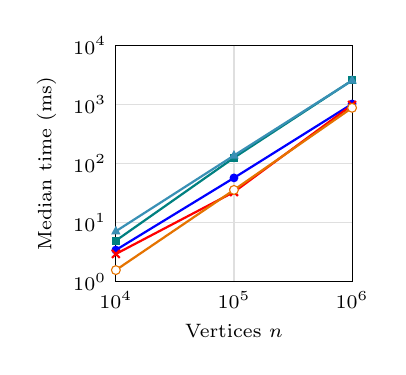
\begin{tikzpicture}[font=\scriptsize]
\draw[gray!25] (0,0.000) -- (3.0,0.000);
\node[left] at (0,0.000) {$10^{0}$};
\draw[gray!25] (0,0.750) -- (3.0,0.750);
\node[left] at (0,0.750) {$10^{1}$};
\draw[gray!25] (0,1.500) -- (3.0,1.500);
\node[left] at (0,1.500) {$10^{2}$};
\draw[gray!25] (0,2.250) -- (3.0,2.250);
\node[left] at (0,2.250) {$10^{3}$};
\draw[gray!25] (0,3.000) -- (3.0,3.000);
\node[left] at (0,3.000) {$10^{4}$};
\draw[gray!25] (0.000,0) -- (0.000,3.0);
\node[below] at (0.000,0) {$10^4$};
\draw[gray!25] (1.500,0) -- (1.500,3.0);
\node[below] at (1.500,0) {$10^5$};
\draw[gray!25] (3.000,0) -- (3.000,3.0);
\node[below] at (3.000,0) {$10^6$};
\draw (0,0) rectangle (3.0,3.0);
\node[below=12pt] at (1.5,0) {Vertices $n$};
\node[rotate=90,above=18pt] at (0,1.5) {Median time (ms)};
\draw[blue, thick] (0.000,0.403) -- (1.500,1.319) -- (3.000,2.258);
\fill[blue] (0.000,0.403) circle (1.6pt);
\fill[blue] (1.500,1.319) circle (1.6pt);
\fill[blue] (3.000,2.258) circle (1.6pt);
\draw[teal, thick] (0.000,0.522) -- (1.500,1.575) -- (3.000,2.557);
\fill[teal] (-0.050,0.472) rectangle (0.050,0.572);
\fill[teal] (1.450,1.525) rectangle (1.550,1.625);
\fill[teal] (2.950,2.507) rectangle (3.050,2.607);
\draw[cyan!70!black, thick] (0.000,0.641) -- (1.500,1.603) -- (3.000,2.555);
\fill[cyan!70!black] (0.000,0.711) -- (-0.060,0.601) -- (0.060,0.601) -- cycle;
\fill[cyan!70!black] (1.500,1.673) -- (1.440,1.563) -- (1.560,1.563) -- cycle;
\fill[cyan!70!black] (3.000,2.625) -- (2.940,2.515) -- (3.060,2.515) -- cycle;
\draw[red, thick] (0.000,0.353) -- (1.500,1.140) -- (3.000,2.245);
\draw[red, thick] (-0.050,0.303) -- (0.050,0.403) (-0.050,0.403) -- (0.050,0.303);
\draw[red, thick] (1.450,1.090) -- (1.550,1.190) (1.450,1.190) -- (1.550,1.090);
\draw[red, thick] (2.950,2.195) -- (3.050,2.295) (2.950,2.295) -- (3.050,2.195);
\draw[orange!90!black, thick] (0.000,0.148) -- (1.500,1.166) -- (3.000,2.209);
\draw[orange!90!black, fill=white] (0.000,0.148) circle (1.6pt);
\draw[orange!90!black, fill=white] (1.500,1.166) circle (1.6pt);
\draw[orange!90!black, fill=white] (3.000,2.209) circle (1.6pt);
\end{tikzpicture}
 &
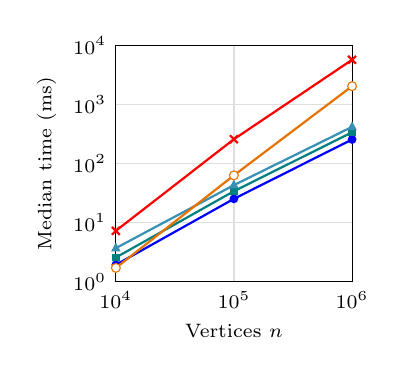
\begin{tikzpicture}[font=\scriptsize]
\draw[gray!25] (0,0.000) -- (3.0,0.000);
\node[left] at (0,0.000) {$10^{0}$};
\draw[gray!25] (0,0.750) -- (3.0,0.750);
\node[left] at (0,0.750) {$10^{1}$};
\draw[gray!25] (0,1.500) -- (3.0,1.500);
\node[left] at (0,1.500) {$10^{2}$};
\draw[gray!25] (0,2.250) -- (3.0,2.250);
\node[left] at (0,2.250) {$10^{3}$};
\draw[gray!25] (0,3.000) -- (3.0,3.000);
\node[left] at (0,3.000) {$10^{4}$};
\draw[gray!25] (0.000,0) -- (0.000,3.0);
\node[below] at (0.000,0) {$10^4$};
\draw[gray!25] (1.500,0) -- (1.500,3.0);
\node[below] at (1.500,0) {$10^5$};
\draw[gray!25] (3.000,0) -- (3.000,3.0);
\node[below] at (3.000,0) {$10^6$};
\draw (0,0) rectangle (3.0,3.0);
\node[below=12pt] at (1.5,0) {Vertices $n$};
\node[rotate=90,above=18pt] at (0,1.5) {Median time (ms)};
\draw[blue, thick] (0.000,0.215) -- (1.499,1.053) -- (3.000,1.807);
\fill[blue] (0.000,0.215) circle (1.6pt);
\fill[blue] (1.499,1.053) circle (1.6pt);
\fill[blue] (3.000,1.807) circle (1.6pt);
\draw[teal, thick] (0.000,0.308) -- (1.499,1.150) -- (3.000,1.898);
\fill[teal] (-0.050,0.258) rectangle (0.050,0.358);
\fill[teal] (1.449,1.100) rectangle (1.549,1.200);
\fill[teal] (2.950,1.848) rectangle (3.050,1.948);
\draw[cyan!70!black, thick] (0.000,0.427) -- (1.499,1.227) -- (3.000,1.967);
\fill[cyan!70!black] (0.000,0.497) -- (-0.060,0.387) -- (0.060,0.387) -- cycle;
\fill[cyan!70!black] (1.499,1.297) -- (1.439,1.187) -- (1.559,1.187) -- cycle;
\fill[cyan!70!black] (3.000,2.037) -- (2.940,1.927) -- (3.060,1.927) -- cycle;
\draw[red, thick] (0.000,0.647) -- (1.499,1.810) -- (3.000,2.819);
\draw[red, thick] (-0.050,0.597) -- (0.050,0.697) (-0.050,0.697) -- (0.050,0.597);
\draw[red, thick] (1.449,1.760) -- (1.549,1.860) (1.449,1.860) -- (1.549,1.760);
\draw[red, thick] (2.950,2.769) -- (3.050,2.869) (2.950,2.869) -- (3.050,2.769);
\draw[orange!90!black, thick] (0.000,0.176) -- (1.499,1.351) -- (3.000,2.484);
\draw[orange!90!black, fill=white] (0.000,0.176) circle (1.6pt);
\draw[orange!90!black, fill=white] (1.499,1.351) circle (1.6pt);
\draw[orange!90!black, fill=white] (3.000,2.484) circle (1.6pt);
\end{tikzpicture}
 &
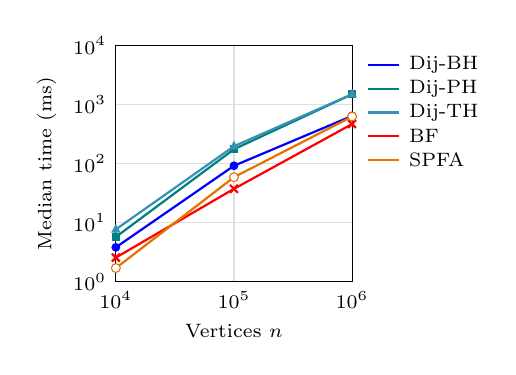
\begin{tikzpicture}[font=\scriptsize]
\draw[gray!25] (0,0.000) -- (3.0,0.000);
\node[left] at (0,0.000) {$10^{0}$};
\draw[gray!25] (0,0.750) -- (3.0,0.750);
\node[left] at (0,0.750) {$10^{1}$};
\draw[gray!25] (0,1.500) -- (3.0,1.500);
\node[left] at (0,1.500) {$10^{2}$};
\draw[gray!25] (0,2.250) -- (3.0,2.250);
\node[left] at (0,2.250) {$10^{3}$};
\draw[gray!25] (0,3.000) -- (3.0,3.000);
\node[left] at (0,3.000) {$10^{4}$};
\draw[gray!25] (0.000,0) -- (0.000,3.0);
\node[below] at (0.000,0) {$10^4$};
\draw[gray!25] (1.500,0) -- (1.500,3.0);
\node[below] at (1.500,0) {$10^5$};
\draw[gray!25] (3.000,0) -- (3.000,3.0);
\node[below] at (3.000,0) {$10^6$};
\draw (0,0) rectangle (3.0,3.0);
\node[below=12pt] at (1.5,0) {Vertices $n$};
\node[rotate=90,above=18pt] at (0,1.5) {Median time (ms)};
\draw[blue, thick] (0.000,0.437) -- (1.500,1.473) -- (3.000,2.106);
\fill[blue] (0.000,0.437) circle (1.6pt);
\fill[blue] (1.500,1.473) circle (1.6pt);
\fill[blue] (3.000,2.106) circle (1.6pt);
\draw[blue, thick] (3.2,2.750) -- (3.6,2.750);
\node[right] at (3.6,2.750) {Dij-BH};
\draw[teal, thick] (0.000,0.569) -- (1.500,1.683) -- (3.000,2.381);
\fill[teal] (-0.050,0.519) rectangle (0.050,0.619);
\fill[teal] (1.450,1.633) rectangle (1.550,1.733);
\fill[teal] (2.950,2.331) rectangle (3.050,2.431);
\draw[teal, thick] (3.2,2.450) -- (3.6,2.450);
\node[right] at (3.6,2.450) {Dij-PH};
\draw[cyan!70!black, thick] (0.000,0.665) -- (1.500,1.721) -- (3.000,2.381);
\fill[cyan!70!black] (0.000,0.735) -- (-0.060,0.625) -- (0.060,0.625) -- cycle;
\fill[cyan!70!black] (1.500,1.791) -- (1.440,1.681) -- (1.560,1.681) -- cycle;
\fill[cyan!70!black] (3.000,2.451) -- (2.940,2.341) -- (3.060,2.341) -- cycle;
\draw[cyan!70!black, thick] (3.2,2.150) -- (3.6,2.150);
\node[right] at (3.6,2.150) {Dij-TH};
\draw[red, thick] (0.000,0.307) -- (1.500,1.180) -- (3.000,2.003);
\draw[red, thick] (-0.050,0.257) -- (0.050,0.357) (-0.050,0.357) -- (0.050,0.257);
\draw[red, thick] (1.450,1.130) -- (1.550,1.230) (1.450,1.230) -- (1.550,1.130);
\draw[red, thick] (2.950,1.953) -- (3.050,2.053) (2.950,2.053) -- (3.050,1.953);
\draw[red, thick] (3.2,1.850) -- (3.6,1.850);
\node[right] at (3.6,1.850) {BF};
\draw[orange!90!black, thick] (0.000,0.174) -- (1.500,1.328) -- (3.000,2.098);
\draw[orange!90!black, fill=white] (0.000,0.174) circle (1.6pt);
\draw[orange!90!black, fill=white] (1.500,1.328) circle (1.6pt);
\draw[orange!90!black, fill=white] (3.000,2.098) circle (1.6pt);
\draw[orange!90!black, thick] (3.2,1.550) -- (3.6,1.550);
\node[right] at (3.6,1.550) {SPFA};
\end{tikzpicture}
 \\
(a) Random sparse ($m\approx5n$) & (b) 2-D grid & (c) Scale-free (BA, $k=3$)
\end{tabular}
\caption{Median running time versus number of vertices (log--log). The label-correcting methods (BF, SPFA) beat Dijkstra on low-diameter graphs (a, c) but scale badly on grids (b).}
\label{fig:scaling}
\end{figure*}

\Cref{tab:main} reports median running times and \cref{fig:scaling} shows
scaling. \Cref{tab:relax} reports the number of edge relaxations per arc, a
hardware-independent measure of work. Dijkstra scans every reachable arc exactly
once, so its value is always $1.00$.

\begin{table}[t]
\centering
\caption{Mean edge relaxations per arc (machine-independent work).}
\label{tab:relax}
\footnotesize
\begin{tabular}{llrrr}
\toprule
Family & $n$ & Dijkstra & BF & SPFA \\
\midrule
Random sparse & $10^4$ & 1.00 & 11.32 & 2.30 \\
 & $10^5$ & 1.00 & 13.02 & 2.45 \\
 & $10^6$ & 1.00 & 16.42 & 2.75 \\
\midrule
2-D grid & $10^4$ & 1.00 & 68.16 & 4.38 \\
 & 99{,}856 & 1.00 & 221.65 & 13.71 \\
 & $10^6$ & 1.00 & 735.07 & 41.65 \\
\midrule
Scale-free (BA) & $10^4$ & 1.00 & 9.99 & 2.41 \\
 & $10^5$ & 1.00 & 11.82 & 2.96 \\
 & $10^6$ & 1.00 & 14.28 & 3.25 \\
\midrule
Random dense & $10^3$ & 1.00 & 7.22 & 2.69 \\
 & 2{,}000 & 1.00 & 7.32 & 2.68 \\
 & 4{,}000 & 1.00 & 6.62 & 2.52 \\
\bottomrule
\end{tabular}

\end{table}

\subsection{Low-diameter graphs: label-correcting methods win in practice}
On random sparse and scale-free graphs, SPFA or Bellman--Ford was the fastest
algorithm at every size. At $10^5$ vertices, Bellman--Ford was $1.7\times$
(sparse) and $2.5\times$ (scale-free) faster than the binary-heap Dijkstra
(Dij-BH). At $10^6$ vertices, the fastest label-correcting method was still
$1.16\times$ (sparse, SPFA) and $1.37\times$ (scale-free, Bellman--Ford)
faster. This
happened even though they did more work. SPFA relaxed each arc $2.3$--$3.3$
times on average and Bellman--Ford $10$--$16$ times
(\cref{tab:relax}). Their work grew only slowly with $n$, which is consistent
with the logarithmic diameter of these graphs. We attribute the wall-clock
advantage to memory behaviour. A Bellman--Ford pass streams through the CSR
arrays sequentially, while each heap operation in Dijkstra touches
$O(\log n)$ scattered memory locations. We did not measure cache misses
directly, so this explanation is a hypothesis.

\subsection{High-diameter graphs: Dijkstra wins decisively}
Grids reverse the picture. SPFA's relaxations per arc grew from $4.4$ at
$n=10^4$ to $13.7$ at $10^5$ and $41.6$ at $10^6$. Bellman--Ford's grew from
$68$ to $222$ to $735$, because the number of passes tracks the graph diameter
($\Theta(\sqrt n)$ on grids). At $10^6$ vertices Dij-BH took 257\,ms, against
2.05\,s for SPFA ($8.0\times$) and 5.75\,s for Bellman--Ford ($22\times$).
SPFA was marginally faster only on the smallest grid. Because SPFA has no
useful worst-case guarantee and degrades badly on grid- and road-like
structure, it is a risky default.

\subsection{Priority queues: simple beats sophisticated}
The lazy-deletion binary heap was the fastest heap-based Dijkstra variant in
every configuration of \cref{tab:main}. Pairing heaps (Dij-PH) were
$1.3$--$2.5\times$ slower and thin heaps (Dij-TH) $1.6$--$2.5\times$ slower,
even though they perform fewer heap operations, since each vertex is inserted
only once. The only exception was the sparsest end of the density sweep
($p\le2\%$), where the pairing heap matched the binary heap to within
$3\%$. The theoretical
$O(m + n\log n)$ advantage of Fibonacci-type heaps did not appear at any size
we tested. This agrees with Larkin et al.~\cite{larkin2014}.

\subsection{Density}
\begin{figure}[t]
\centering
\resizebox{\columnwidth}{!}{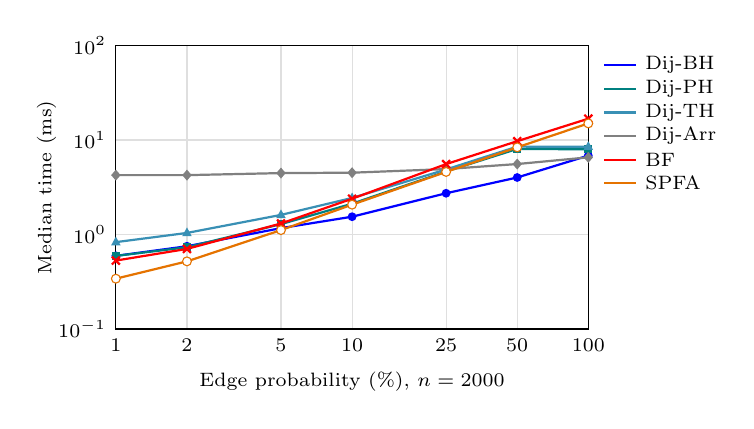
\begin{tikzpicture}[font=\scriptsize]
\draw[gray!25] (0,0.000) -- (6.0,0.000);
\node[left] at (0,0.000) {$10^{-1}$};
\draw[gray!25] (0,1.200) -- (6.0,1.200);
\node[left] at (0,1.200) {$10^{0}$};
\draw[gray!25] (0,2.400) -- (6.0,2.400);
\node[left] at (0,2.400) {$10^{1}$};
\draw[gray!25] (0,3.600) -- (6.0,3.600);
\node[left] at (0,3.600) {$10^{2}$};
\draw[gray!25] (0.000,0) -- (0.000,3.6);
\node[below] at (0.000,0) {1};
\draw[gray!25] (0.903,0) -- (0.903,3.6);
\node[below] at (0.903,0) {2};
\draw[gray!25] (2.097,0) -- (2.097,3.6);
\node[below] at (2.097,0) {5};
\draw[gray!25] (3.000,0) -- (3.000,3.6);
\node[below] at (3.000,0) {10};
\draw[gray!25] (4.194,0) -- (4.194,3.6);
\node[below] at (4.194,0) {25};
\draw[gray!25] (5.097,0) -- (5.097,3.6);
\node[below] at (5.097,0) {50};
\draw[gray!25] (6.000,0) -- (6.000,3.6);
\node[below] at (6.000,0) {100};
\draw (0,0) rectangle (6.0,3.6);
\node[below=12pt] at (3.0,0) {Edge probability (\%), $n=2000$};
\node[rotate=90,above=18pt] at (0,1.8) {Median time (ms)};
\draw[blue, thick] (0.000,0.929) -- (0.903,1.051) -- (2.097,1.281) -- (3.000,1.426) -- (4.194,1.724) -- (5.097,1.924) -- (6.000,2.202);
\fill[blue] (0.000,0.929) circle (1.6pt);
\fill[blue] (0.903,1.051) circle (1.6pt);
\fill[blue] (2.097,1.281) circle (1.6pt);
\fill[blue] (3.000,1.426) circle (1.6pt);
\fill[blue] (4.194,1.724) circle (1.6pt);
\fill[blue] (5.097,1.924) circle (1.6pt);
\fill[blue] (6.000,2.202) circle (1.6pt);
\draw[blue, thick] (6.2,3.350) -- (6.6,3.350);
\node[right] at (6.6,3.350) {Dij-BH};
\draw[teal, thick] (0.000,0.928) -- (0.903,1.038) -- (2.097,1.332) -- (3.000,1.591) -- (4.194,2.000) -- (5.097,2.287) -- (6.000,2.282);
\fill[teal] (-0.050,0.878) rectangle (0.050,0.978);
\fill[teal] (0.853,0.988) rectangle (0.953,1.088);
\fill[teal] (2.047,1.282) rectangle (2.147,1.382);
\fill[teal] (2.950,1.541) rectangle (3.050,1.641);
\fill[teal] (4.144,1.950) rectangle (4.244,2.050);
\fill[teal] (5.047,2.237) rectangle (5.147,2.337);
\fill[teal] (5.950,2.232) rectangle (6.050,2.332);
\draw[teal, thick] (6.2,3.050) -- (6.6,3.050);
\node[right] at (6.6,3.050) {Dij-PH};
\draw[cyan!70!black, thick] (0.000,1.103) -- (0.903,1.220) -- (2.097,1.449) -- (3.000,1.664) -- (4.194,2.026) -- (5.097,2.316) -- (6.000,2.315);
\fill[cyan!70!black] (0.000,1.173) -- (-0.060,1.063) -- (0.060,1.063) -- cycle;
\fill[cyan!70!black] (0.903,1.290) -- (0.843,1.180) -- (0.963,1.180) -- cycle;
\fill[cyan!70!black] (2.097,1.519) -- (2.037,1.409) -- (2.157,1.409) -- cycle;
\fill[cyan!70!black] (3.000,1.734) -- (2.940,1.624) -- (3.060,1.624) -- cycle;
\fill[cyan!70!black] (4.194,2.096) -- (4.134,1.986) -- (4.254,1.986) -- cycle;
\fill[cyan!70!black] (5.097,2.386) -- (5.037,2.276) -- (5.157,2.276) -- cycle;
\fill[cyan!70!black] (6.000,2.385) -- (5.940,2.275) -- (6.060,2.275) -- cycle;
\draw[cyan!70!black, thick] (6.2,2.750) -- (6.6,2.750);
\node[right] at (6.6,2.750) {Dij-TH};
\draw[gray, thick] (0.000,1.954) -- (0.903,1.954) -- (2.097,1.980) -- (3.000,1.985) -- (4.194,2.031) -- (5.097,2.095) -- (6.000,2.180);
\fill[gray] (0.000,2.024) -- (-0.060,1.954) -- (0.000,1.884) -- (0.060,1.954) -- cycle;
\fill[gray] (0.903,2.024) -- (0.843,1.954) -- (0.903,1.884) -- (0.963,1.954) -- cycle;
\fill[gray] (2.097,2.050) -- (2.037,1.980) -- (2.097,1.910) -- (2.157,1.980) -- cycle;
\fill[gray] (3.000,2.055) -- (2.940,1.985) -- (3.000,1.915) -- (3.060,1.985) -- cycle;
\fill[gray] (4.194,2.101) -- (4.134,2.031) -- (4.194,1.961) -- (4.254,2.031) -- cycle;
\fill[gray] (5.097,2.165) -- (5.037,2.095) -- (5.097,2.025) -- (5.157,2.095) -- cycle;
\fill[gray] (6.000,2.250) -- (5.940,2.180) -- (6.000,2.110) -- (6.060,2.180) -- cycle;
\draw[gray, thick] (6.2,2.450) -- (6.6,2.450);
\node[right] at (6.6,2.450) {Dij-Arr};
\draw[red, thick] (0.000,0.869) -- (0.903,1.017) -- (2.097,1.340) -- (3.000,1.654) -- (4.194,2.094) -- (5.097,2.385) -- (6.000,2.671);
\draw[red, thick] (-0.050,0.819) -- (0.050,0.919) (-0.050,0.919) -- (0.050,0.819);
\draw[red, thick] (0.853,0.967) -- (0.953,1.067) (0.853,1.067) -- (0.953,0.967);
\draw[red, thick] (2.047,1.290) -- (2.147,1.390) (2.047,1.390) -- (2.147,1.290);
\draw[red, thick] (2.950,1.604) -- (3.050,1.704) (2.950,1.704) -- (3.050,1.604);
\draw[red, thick] (4.144,2.044) -- (4.244,2.144) (4.144,2.144) -- (4.244,2.044);
\draw[red, thick] (5.047,2.335) -- (5.147,2.435) (5.047,2.435) -- (5.147,2.335);
\draw[red, thick] (5.950,2.621) -- (6.050,2.721) (5.950,2.721) -- (6.050,2.621);
\draw[red, thick] (6.2,2.150) -- (6.6,2.150);
\node[right] at (6.6,2.150) {BF};
\draw[orange!90!black, thick] (0.000,0.639) -- (0.903,0.859) -- (2.097,1.256) -- (3.000,1.579) -- (4.194,1.995) -- (5.097,2.307) -- (6.000,2.611);
\draw[orange!90!black, fill=white] (0.000,0.639) circle (1.6pt);
\draw[orange!90!black, fill=white] (0.903,0.859) circle (1.6pt);
\draw[orange!90!black, fill=white] (2.097,1.256) circle (1.6pt);
\draw[orange!90!black, fill=white] (3.000,1.579) circle (1.6pt);
\draw[orange!90!black, fill=white] (4.194,1.995) circle (1.6pt);
\draw[orange!90!black, fill=white] (5.097,2.307) circle (1.6pt);
\draw[orange!90!black, fill=white] (6.000,2.611) circle (1.6pt);
\draw[orange!90!black, thick] (6.2,1.850) -- (6.6,1.850);
\node[right] at (6.6,1.850) {SPFA};
\end{tikzpicture}
}
\caption{Effect of edge density at fixed $n=2000$ (median time, log scale).}
\label{fig:density}
\end{figure}
\Cref{fig:density} varies the edge probability at $n=2000$. At $p\le 2\%$
(average degree $\le 40$), SPFA was fastest, at $0.34$\,ms versus $0.60$\,ms
for Dij-BH at $p=1\%$. The two were roughly tied at $p=5\%$, and from
$p=10\%$ upwards Dij-BH was the fastest heap-based method. At $p=50\%$ it was
$2.1\times$ faster than SPFA and $2.4\times$ faster than Bellman--Ford. The
$O(n^2)$ array version of Dijkstra became competitive as the graph approached
completeness. At $p=100\%$ it took 6.56\,ms against 6.84\,ms for Dij-BH,
confirming the textbook advice that the array variant suits dense graphs.

\subsection{Point-to-point queries: A* depends on heuristic quality}
\begin{table}[t]
\centering
\caption{Point-to-point queries on a $1000\times1000$ grid with weights $U[w_{\min},1000]$ and heuristic $w_{\min}\cdot$Manhattan distance (20 random pairs each).}
\label{tab:astar}
\footnotesize
\setlength{\tabcolsep}{4pt}
\begin{tabular}{rrrrrr}
\toprule
$w_{\min}$ & \multicolumn{2}{c}{Median time (ms)} & \multicolumn{2}{c}{Mean arcs scanned ($\times 10^3$)} & Speed-up \\
\cmidrule(lr){2-3}\cmidrule(lr){4-5}
 & Dijkstra & A* & Dijkstra & A* & \\
\midrule
1 & 120 & 119 & 2{,}182 & 2{,}176 & 1.0$\times$ \\
100 & 112 & 86.9 & 2{,}181 & 1{,}571 & 1.3$\times$ \\
250 & 103 & 50.7 & 2{,}174 & 1{,}090 & 2.0$\times$ \\
500 & 91.5 & 24.7 & 2{,}167 & 713 & 3.7$\times$ \\
750 & 85.7 & 18.8 & 2{,}158 & 537 & 4.6$\times$ \\
900 & 85.2 & 14.7 & 2{,}153 & 476 & 5.8$\times$ \\
\bottomrule
\end{tabular}

\end{table}
For $s$--$t$ queries on the $10^6$-vertex grid, we varied the minimum edge
weight $w_{\min}$. The Manhattan heuristic is scaled by $w_{\min}$, so a larger
$w_{\min}$ gives a tighter lower bound (\cref{tab:astar}). With $w_{\min}=1$
and weights averaging about $500$, the heuristic carries almost no information
and A* scans as many arcs as Dijkstra, with no speed-up. As $w_{\min}$ grows,
the scanned arcs fall from $2.18$ million to $0.48$ million and the speed-up
rises to $5.8\times$. A* is therefore not inherently faster. Its benefit is
determined entirely by how tight the heuristic is.

%% ------------------------------------------------------------------
\section{Discussion and Practical Guidelines}

Our measurements support the following guidelines for non-negative weights.
\begin{enumerate}
  \item \textbf{Use Dijkstra with a lazy binary heap as the default.} It was
        never far from the best (at most $2.5\times$ slower, on the
        $10^5$-vertex scale-free graph), it was the clear winner on high-diameter and dense
        graphs, and its $O(m\log n)$ bound protects against bad inputs.
  \item \textbf{Do not reach for Fibonacci-type heaps.} Pairing and thin heaps
        with \textsc{decrease-key} were consistently slower in our tests.
  \item \textbf{SPFA/Bellman--Ford can be faster on low-diameter graphs}, such
        as random or social-network-like graphs, by up to $2.5\times$ in our
        experiments. They become dangerous on grid- or road-like graphs, where
        their work grows super-linearly. Use them only when the structure is
        known or negative weights force the choice.
  \item \textbf{For very dense graphs ($p\to1$), the $O(n^2)$ array version is
        competitive} and simpler.
  \item \textbf{For point-to-point queries, invest in the heuristic.} A* with a
        weak lower bound is just Dijkstra with overhead. With a tight bound it
        gave up to $5.8\times$ in our tests. Landmark-based
        heuristics~\cite{goldberg2005} or preprocessing such as contraction
        hierarchies~\cite{geisberger2008} are the next step.
\end{enumerate}
These findings also qualify a common claim. The relative performance of
Dijkstra and label-correcting methods is not a fixed percentage. It depends
strongly on graph diameter and density, and can reverse direction between
graph families of the same size.

%% ------------------------------------------------------------------
\section{Threats to Validity and Limitations}
\label{sec:limits}

\emph{Single platform.} All timings come from one laptop CPU. Absolute numbers
will differ on other hardware, which is why we also report relaxation counts.
\emph{Synthetic graphs.} We use generated graphs with uniform integer weights.
Real road networks (e.g.\ DIMACS~\cite{dimacs2009}) have correlated weights and
geometric structure that may favour A* and hurt SPFA more than our grids do.
\emph{Non-negative weights only.} Dijkstra does not apply to negative weights,
so the main advantage of Bellman--Ford/SPFA is not exercised. We compare the
algorithms on the instances where all of them are correct.
\emph{Implementation choices.} Library heaps (\texttt{pb\_ds}) may not be the
fastest available implementations of their data structures. Radix heaps, Dial's
buckets and $\Delta$-stepping were not included.
\emph{Recent theory.} We did not implement the algorithm of
Duan et al.~\cite{duan2025}. A faithful, tuned implementation and its comparison
with the baselines here is the natural next step.

%% ------------------------------------------------------------------
\section{Conclusion}

We presented a reproducible comparison of Dijkstra's algorithm with
label-correcting SSSP methods on four graph families up to $10^6$ vertices. No
single algorithm dominated. Label-correcting methods were faster on
low-diameter graphs despite doing more work. Dijkstra was far more robust,
winning by up to $22\times$ on grids. A plain binary heap beat theoretically
superior heaps, and A*'s benefit depended entirely on its heuristic. Future
work includes real road networks from the DIMACS challenge, hardware-counter
measurements to test the cache hypothesis, negative-weight instances, parallel
methods such as $\Delta$-stepping, and a tuned implementation of the
sorting-barrier-breaking algorithm of Duan et al.~\cite{duan2025} to test
whether its asymptotic gains appear in practice.

\section*{Reproducibility}
\label{sec:repro}
Source code, raw measurements (\texttt{results/raw.csv}), the aggregation script
and the scripts that generate every table and figure in this paper are available
at \url{https://github.com/theUsamasaleem/sssp-empirical-study}. The
command \texttt{./run\_all.sh \&\& python3 analyze.py} regenerates all results.

\bibliographystyle{IEEEtran}
\bibliography{refs}

\end{document}
